\documentclass[12pt,a4paper,twoside]{book}


\usepackage[utf8]{inputenc}
\usepackage[a4paper,inner=3.5cm,outer=2.5cm]{geometry}

\usepackage[titletoc,title,toc,page]{appendix}
\usepackage{verbatim}
\usepackage{placeins}
\usepackage{listings}
\usepackage{hyperref}
\usepackage[italian]{babel}
\usepackage{tikz}
\usepackage{parskip}
\usepackage{newpxtext,newpxmath}
\usepackage{graphicx}
\usepackage{blindtext}
\usepackage{chngcntr}
\counterwithin{table}{chapter}
\usepackage{spverbatim}
\usepackage{newlfont}
\usepackage{fancyhdr}
\usepackage{indentfirst}
\usepackage[utf8]{inputenc}
\usepackage{float}
\usepackage{hyperref}
\usepackage[capitalize,noabbrev]{cleveref}
\usepackage{soul}
\usepackage[font=footnotesize,labelfont=bf]{caption}

\usepackage{multirow}
\usepackage{hyphenat}


%start roba script
\usepackage{xcolor}
\usepackage{listings}

% --- SCHEMA COLORI "MODERN LIGHT" ---
\definecolor{code_keyword}{RGB}{215, 58, 73}   % Rosso scuro elegante
\definecolor{code_string}{RGB}{3, 47, 98}    % Blu notte
\definecolor{code_comment}{RGB}{106, 115, 125} % Grigio ardesia per i commenti
\definecolor{code_bg}{RGB}{250, 251, 252}      % Bianco ghiaccio (quasi impercettibile)
\definecolor{code_frame}{RGB}{225, 228, 232}   % Grigio chiaro per i bordi

\lstset{
    backgroundcolor=\color{code_bg},   
    commentstyle=\color{code_comment}\itshape,
    keywordstyle=\color{code_keyword}\bfseries,
    stringstyle=\color{code_string},
    basicstyle=\ttfamily\small\color{black!85}, % Testo quasi nero, meno aggressivo
    breakatwhitespace=false,         
    breaklines=true,                 
    captionpos=b,                    
    keepspaces=true,                 
    numbers=none,       
    tabsize=4,
    frame=single,                    % Box completo
    rulecolor=\color{code_frame},    % Colore del bordo discreto
    framerule=0.8pt,                 % Spessore bordo sottile
    xleftmargin=5pt,                 % Padding interno
    xrightmargin=5pt,
    % --- FIX CARATTERI SPECIALI ---
    extendedchars=true,
    literate=
        {á}{{\'a}}1 {é}{{\'e}}1 {í}{{\'i}}1 {ó}{{\'o}}1 {ú}{{\'u}}1
        {à}{{\`a}}1 {è}{{\`e}}1 {ì}{{\`i}}1 {ò}{{\`o}}1 {ù}{{\`u}}1
        {→}{{$\rightarrow$}}1 {—}{{---}}1 {°}{{$^\circ$}}1
}


% end roba script


\hyphenation{mate-mati-ca recu-perare}

\usepackage{lscape} 

\usepackage[
    backend=biber,
    style=numeric,   
    sorting=nyt,        
    maxbibnames=10,
    maxcitenames=2,
    hyperref=true       
]{biblatex}
\addbibresource{refs.bib}  

\newcommand{\rom}[1]{\uppercase\expandafter{\romannumeral #1\relax}}

\usepackage{pdfpages}

\begin{document}
% Per spostare i vari elementi più su o più giù gioca con i valori di vspace che ci sono tra uno e l'altro
\pagestyle{empty}
\newgeometry{
    left=20mm,
    right=20mm,
    top=20mm,
    bottom=20mm
}

\begin{titlepage}

\begin{center}

% marchio di ateneo

\includegraphics[width=6.5cm,height=4.7cm]{img/marchio-di-ateneo.png}

\vspace{10mm}

% \large is 12pt
{\large{\bf{Dipartimento di }}} 

\vspace{5mm}

% \Large is 14.4pt
{\Large{\bf{Corso di Laurea in }}}

\vspace{15mm}

{\Huge{\bf Titolo della tesi }}\\
\vspace{3mm}
{\Huge{\bf anche su più}}\\
\vspace{3mm}
{\Huge{\bf righe }}\\
\vspace{3mm}

\end{center}

\vspace{10mm}

\begin{minipage}[t]{0.40\textwidth}
{\Large{\bf Relatore: \\ Chiar.mo Prof.\\ Nome Cognome}}

\vspace{3mm}

{\Large{\bf Correlatore: \\ Chiar.mo Prof.\\ Nome Cognome}}
\end{minipage}
\hfill
\begin{minipage}[t]{0.40\textwidth}\raggedleft
{\Large{\bf Presentata da: \\ Nome Cognome}}
\end{minipage}

\vspace{30mm}

\rule[0.5cm]{15.8cm}{0.6mm}

\begin{center}
{\large{\bf Sessione mese anno \\}}
{\large{\bf Anno Accademico 20xx/20xx\\}}
\end{center}

\end{titlepage}

\restoregeometry
\newpage
\begin{center}
    (DA FARE ALLA FINE)\\
    5 parole chiave per caratterizzare il contenuto della dissertazione:\\ (se non ti piacciono così sparse puoi anche semplicemente scriverle su una riga sola)
\end{center}

% https://tex.stackexchange.com/questions/26538/words-scattered-randomly-in-on-coverpage
\begin{tikzpicture}[overlay,remember picture,shift=(current page.center)]
\pgfmathsetseed{3}


\foreach [count=\count] \word in {Parola 1, parola 2, parola 3, parola 4, parola 5} {
\node [
    xshift={(mod(\count,3)-1)*(\paperwidth/4)},
    yshift={(mod(\count,7)-3)*(\paperwidth/6)},
    xshift=rand*4cm,
    yshift=rand*2cm,
    % rotate=rand*35,
    % opacity=rnd*0.5+0.125,
    font=\large] {\word};
}
\end{tikzpicture}
\newpage

\topmargin=6.5cm
\begin{flushright}
\emph{
\LARGE{La dedica}\\\vspace{2mm}
\LARGE{anche quella se vuoi}\\\vspace{3mm} 
\LARGE{su più righe} 
}
\end{flushright}
\newpage~\newpage
\pagenumbering{gobble}
\chapter*{Abstract}
Abstract qui (ti consiglio di farlo alla fine)

\topmargin=-1cm
\tableofcontents
\thispagestyle{empty}
\listoftables
\thispagestyle{empty}
\listoffigures
\thispagestyle{empty}
\newpage~\newpage


\pagenumbering{arabic}
\setcounter{chapter}{0}
\raggedbottom
\chapter*{Introduzione} \label{chap:intro}
\addcontentsline{toc}{chapter}{Introduzione}
\chaptermark{Introduzione}

\pagestyle{plain}
\setcounter{page}{1}
A supportare la maggior parte delle infrastrutture di rete troviamo i protocolli 802.3 e 802.11, ethernet standard e WiFi rispettivamente, protocolli che si occupano di gestire il livello 1 (livello fisico) e il livello 2 (livello di data link) della pila protocollare, attraverso una semantica di comunicazione di tipo \textit{best-effort} essi non forniscono garanzie sulla ricezione dei frame, ma il compito viene delegato ai livelli superiori. 
\\
Per questi motivi viene introdotto da parte dell' 802.1 Time-Sensitive Networking Task Group, a partire dagli standard definiti dal protocollo 802.1Q, un insieme di standard e strumenti per fornire comunicazioni mediante reti 802 in grado garantire il trasferimento dei pacchetti in maniera deterministica e affidabile. \cite{TSN_group}
\\
\subsection*{Concetti preliminari}
\begin{itemize}
    \item \textbf{VLAN}: Raggruppamento logico di risorse di rete connesse ad una porta su uno switch, permettono suddivisione del dominio di broadcast e segmentazione di una LAN
    \item \textbf{Bridge}: Un bridge è un dispositivo che opera a livello 2 OSI e permette di connettere e filtrare traffico tra 2 o più segmenti di rete. Come le VLAN favoriscono la segmentazione, diminuendo quindi il dominio di collisione, sono fondamentali per supportare l'interoperabilità tra diverse tecnologie (Ethernet \& Wifi) 
    \item \textbf{Access Link}: Un access link appartiene, e trasporta traffico appartenente, ad una sola VLAN, il traffico è in formato "nativo" ovvero non contiene informazioni riguardo la VLAN ed il collegamento avviene tra l'end device e l'access port. Il dispositivo collegato ad un access port non ha visibilità della VLAN ma "vede" un unico dominio di broadcast
    \item \textbf{Trunk Link}: Un trunk link appartiene, e trasporta traffico appartenente, a più VLAN, connette quindi dispositivi che "comprendono" il concetto di VLAN, solitamente uno switch o un router
    \item \textbf{VLAN tagging}: permette allo switch di aggiungere ai frame (Livello 2) informazioni riguardo la VLAN, così facendo altri dispositivi in grado di "capire" le VLAN sapranno cosa fare con quel frame, il tag verrà rimosso prima di mandare il frame all'end device \cite{VLAN_tagging}
    \item \textbf{SDN}: Insieme di meccanismi che permette di disaccoppiare il control plane (scelte di routing, topologia di rete, gestione policy) dal data plane, un approccio del genere porta ad infrastruttura programmabile e scalabile centralizzata \cite{Software_Defined_Networking_for_Organizations_Network_Automation}
\end{itemize}
\chapter{Caratteristiche e obiettivi di TSN \& WiFi 7}\label{chap:cap1}




\section{Sincronizzazione temporale}
Uno dei requisiti fondamentali per una rete deterministica è una visione condivisa e universale del tempo, TSN utilizza lo standard IEEE 802.1AS o gPTP - \textit{Generalized Precision Time Protocol}, esso definisce un meccanismo di sincronizzazione del clock basato su IEEE 1588.
\\
Il Precision Time Protocol una volta eletto un GM - \textit{GrandMaster}, ovvero il dispositivo con la sorgente temporale più precisa, utilizza frame Ethernet per sincronizzare il clock dei dispositivi della rete utilizzando un approccio GrandMaster - Slave mediante messaggi di \texttt{Sync}, al quale gli Slave risponderanno con richieste per informazioni temporali aggiuntive, a queste il GM risponderà con messaggi di \texttt{Follow-Up} e \texttt{Delay-Resp} che permettono agli Slave di calcolare la differenza dei loro orologi rispetto a quella del GM e avere quindi una visione condivisa del tempo.
\\
Per estendere i servizi offerti da 802.1AS in reti wireless sarà necessario l'utilizzo di protocolli come TM - \textit{Timing Measurement}  o FTM - \textit{Fine Timing Measurement} che nascono come standard per misurare con precisione la distanza tra un STA e un AP sfruttando RTT, esistono in letteratura \cite{TSN_FTM} soluzioni che propongono un mapping tra gPTP e FTM. I timestamp ottenuti tramite lo scambio di messaggi IEEE 802.1AS sul lato cablato vengono correlati con le misurazioni del tempo di volo, ToF - \textit{Time of Flight}, effettuate tramite il protocollo FTM sul lato wireless.
\\
Questo processo permette di compensare le variazioni del mezzo trasmissivo e di estendere il dominio di sincronizzazione TSN ai nodi mobili.
\section{Latenza Limitata e 0 perdite causate da congestione}
Uno degli obiettivi di TSN è quello di garantire bassa latenza e azzerare le perdite di frame causate dal congestionamento della rete, per rispettare questi vincoli si utilizzano diversi meccanismi basati sui concetti di schedulazione,modellazione del traffico e prelazione dei frame. 
\\
Se nel paradigma \textit{best-effort} abbiamo una semantica di gestione del medium e dei nodi di inoltro del tipo \emph{“Fai ciò che dice il pacchetto appena lo ricevi”}, \cite{intro_to_TSN} in TSN la necessità di determinismo e affidabilità \ref{fig:tsn_obiettivi}, porta ad una semantica: \emph{“Fai ciò che dice il pacchetto quando lo dice il pacchetto”}.
\\
Alla base di tutti gli standard definiti ritroviamo il concetto di \textit{classe di traffico}, che permette di suddividere per l'appunto, il traffico, in diversi livelli di priorità, utilizzati poi dagli algoritmi di accodamento \ref{algoritmi_accodamento}.
\\
Un nodo di inoltro è un dispositivo che riceve un frame su una data porta in ingresso e lo invia su una (o più) porte in uscita, in TSN ad ogni porta in uscita è associata una coda, la quale mappa il concetto di classe di traffico, essa dovrà essere gestita in maniera opportuna: un dato algoritmo dovrà selezionare il frame  \textit{“giusto”} e inoltrarlo.
\\
Un principio cardine nella gestione delle code è quello del “mai un buffer vuoto” \cite{intro_to_TSN} che porta al seguente requisito per una rete TSN: 
\begin{center}
    \emph{“Per ogni flusso che attraversa un nodo di inoltro, viene bufferizzata una quantità di dati sufficiente a garantire che non venga mai persa un'opportunità di trasmissione per quel flusso, a meno che la sorgente stessa non rallenti o si interrompa”}
\end{center}
Idealmente data una coda vorremmo che la frequenza dei pacchetti in ingresso fosse uguale a quella dei pacchetti in uscita, dato che se ciò non accade per una durata temporale sufficiente potremmo riscontrare perdite causate dalla congestione \cite{congestion_avoidance_and_control}, che TSN cerca di abbattere. 
\\ 
Frequenze “disaccoppiate” sono causate da un jitter elevato che a sua volta può essere causato da:
\begin{itemize}
    \item Variazioni nel processamento per l'inoltro del frame 
    \item Algoritmi di accodamento che causano “raffiche” o “intervalli” nella trasmissione dei frame
    \item Sorgenti di trasmissione non coordinate
\end{itemize}

\begin{figure}[h]
    \centering
    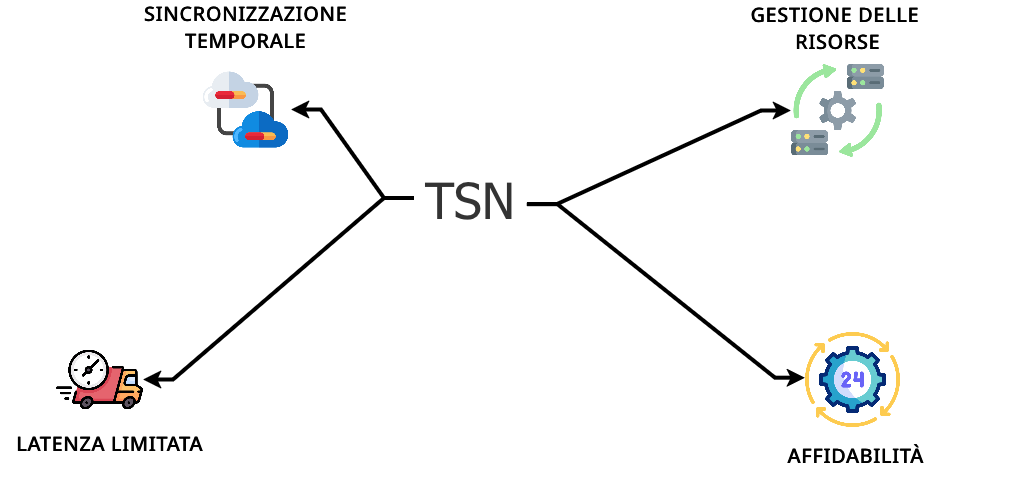
\includegraphics[width=0.8\textwidth]{img/tsn_obiettivi.png}
    \caption{Obiettivi principali di TSN}
    \label{fig:tsn_obiettivi}
\end{figure}

\subsection{Algoritmi di accodamento}\label{algoritmi_accodamento}
Tutti gli algoritmi che verranno presi in esame appartengono allo standard 802.1, principalmente 802.1Q, Bridges e Bridges Networks, dove viene introdotto il concetto di VLAN tagging \cite{vlan_tagging}, questo meccanismo e, nello specifico i 3 bit di PCP - \textit{Priority Code Point} permettono di supportare l'astrazione di classe di traffico.

\begin{figure}[H]
    \centering
    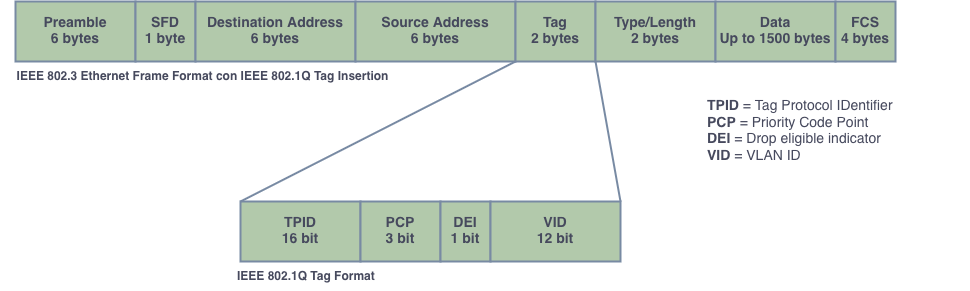
\includegraphics[width=1\textwidth]{img/8021q.png}
    \caption{IEEE 802.3 Ethernet Frame Format con IEEE 802.1Q Tag Insertion}
    \label{fig:pcp}
\end{figure}

Come è possibile osservare in figura \ref{fig:pcp} nel campo Tag introdotto dallo standard 802.1Q sono presenti:
\begin{enumerate}
    \item \textbf{TPID - Tag Protocol Identifier}: 16 bit che identificano il frame come frame VLAN-tagged, il valore è 0x8100
    \item \textbf{PCP - Priority Code Point}: 3 bit che definiscono la priorità del frame riferendosi ad i CoS - \textit{Class of Service} definiti nello standard IEEE 802.1p
    \item \textbf{DEI - Drop Eligible Indicator}: Originariamente denominanto CFI - \textit{Canonical Format Indicator}, 1 bit che indica se il frame può essere eliminato in caso di congestione
    \item \textbf{VID - VLAN Identifier}: 12 bit che identificano la VLAN a cui il frame appartiene
\end{enumerate}

\subsubsection{TAS - Time Aware Shaper}
IEEE 802.1Qbv associa ad ogni classe di traffico presente su una porta in uscita una pianificazione ciclica definita dalla GCL - \textit{Gate Control List}, in cui vengono specificati gli istanti temporali in cui una determinata classe può essere trasmessa, e quindi il gate è aperto.
\\
Questo approccio “consapevole del tempo” richiede l'utilizzo di un clock condiviso che permette di operare con una granularità fino a 1 ns, ciò però è piuttosto oneroso a livello computazionale e infrastrutturale, in reti in cui è necessaria flessibilità, scalabilità ed è presente un traffico sporadico e non programmato, è spesso impraticabile, per questi casi introdurremo successivamente ATS. 
\\
TAS inoltre è in grado di gestire l'apertura di molteplici gate in contemporanea, favorendo il traffico critico, e implementa meccanismi di previsione per capire se riuscirà a inviare l'intero frame prima della chiusura del gate.
\subsubsection{CBS - Credit Base Shaper}
IEEE 802.1Qav, introdotto inizialmente per gestire i flussi multimediali si pone l'obiettivo principale di linearizzare il traffico, andando a ridurre le raffiche e gli intervalli, utilizzando un modello a credito.
Ad ogni coda è associato un credito che viene accumulato quando questa è inattiva, e consumato quando avviene la trasmissione.
\subsubsection{CQF - Cyclic Queuing Forwarding} 
IEEE 802.1Qch come TAS utilizza una pianificazione ciclica per la trasmissione, ma quest'ultima avviene anche per le porte in ingresso, il risultato è un pattern trasmissivo regolare senza le complicazioni introdotte da TAS, in quanto i frame si “spostano in gruppi”.
\subsubsection{Frame Preemption}
802.1Qbu e 802.3br permettono di definire due tipi di code:
\begin{itemize}
    \item \textbf{Express}: I frame in queste code possono causare la prelazione di frame in code \textit{preemptable}
    \item \textbf{Preemptable}: La trasmissione dei frame appartenenti a queste code può essere prelazionata per favorire traffico prioritario, la trasmissione riprenderà dopo la fine dei pacchetti critici
\end{itemize}
L'utilizzo di questi meccanismi di prelazione riduce l'interferenza apportata dal traffico non critico in una rete deterministica, questo studio \cite{tsn_exp} mostra come sia possibile ottenere un miglioramento di circa il 91\% sulla latenza massima e del 94,5\% sul jitter.
\\
In figura \ref{fig:frame_preemption} è mostrata la differenza nella gestione del traffico con e senza frame preemption, si può notare come senza questo meccanismo, il traffico critico subisce un ritardo causato dalla trasmissione di frame non critici, mentre con la prelazione, il traffico critico viene trasmesso immediatamente a meno di un delay \textit{d} introdotto dai meccanismi di prelazione.

\begin{figure}[H]
    \centering
    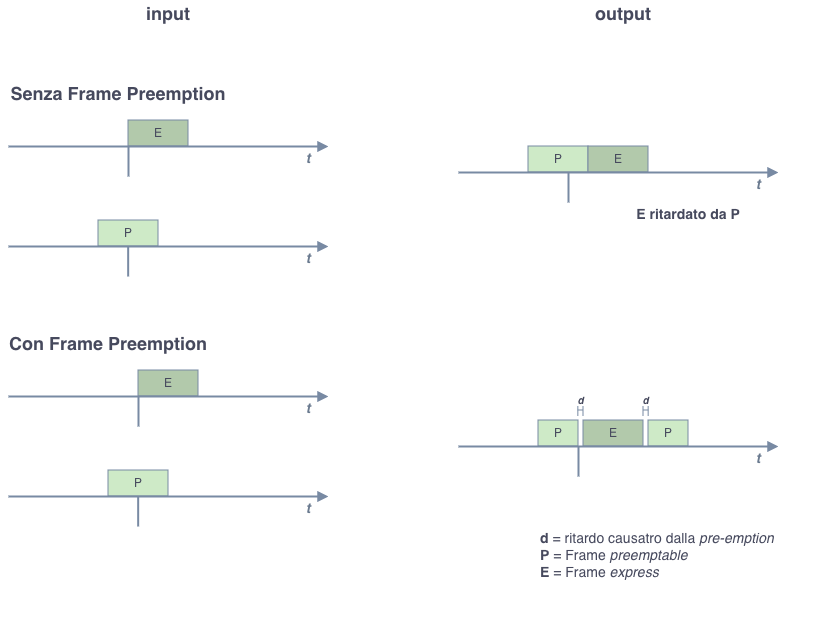
\includegraphics[width=0.8\textwidth]{img/frameprem.png}
    \caption{Differenza nella gestione del traffico con e senza frame preemption}
    \label{fig:frame_preemption}
\end{figure}

\subsubsection{ATS - Asynchronous Traffic Shaping}
Nella descrizione di TAS sono state evidenziate le criticità in contesti dove il traffico non è periodico, IEEE 802.1Qcr si pone l'obiettivo di fornire modellazione e pianificazione del traffico senza la necessità di un elevato accoppiamento temporale (clock condiviso), sfruttando un approccio event-driven \cite{ats}, a ogni pacchetto in ingresso viene assegnato un tempo di trasmissione.
Ciò avviene tramite una macchina a stati che mostrata in figura \ref{fig:ats},descrive i diversi stati possibili e gli eventi che possono scatenare una transizione tra di essi.
\\
I 2 principali protocolli sono:
\begin{itemize}
    \item \textbf{UBS -  Urgency Based Scheduler}: Garantisce priorità al traffico critico
    \item \textbf{TBE - Token Bucket Emulation}:  Garantisce una velocità media di trasmissione ed evita raffiche 
\end{itemize}

\begin{figure}[H]
    \centering
    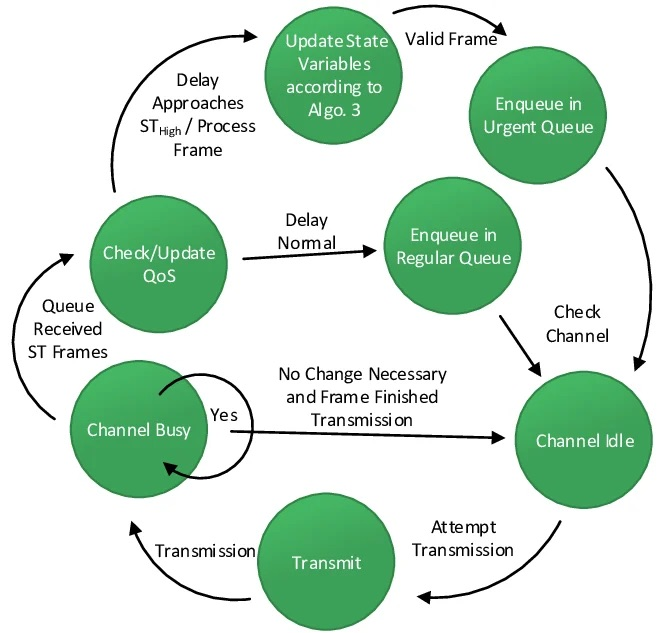
\includegraphics[width=0.6\textwidth]{img/Asynchronous-Traffic-Shaping-ATS-state-machine-illustrating-the-states-and-transitional.jpeg}
    \caption{Macchina a stati di ATS, fonte: \cite{ats}}
    \label{fig:ats}
\end{figure}

Questo algoritmo è ideale per situazioni ibride in cui coesistono sia traffico periodico che sporadico, per una comparazione dettagliata tra ATS e TAS si veda \cite{ats_performance}
\section{Affidabilità}
Un elevato grado di affidabilità è richiesto per reti TSN, non essendo possibile basarsi su ritrasmissioni dei pacchetti data la natura \emph{time-sensitive} del traffico, si introducono diversi meccanismi:
\subsection{FRER - 	Frame Replication and Elimination for Reliability }
Lo standard 802.1CB, permette di replicare i frame attraverso diversi percorsi, successivamente eliminando i duplicati.
Ogni flusso duplicato viene chiamato \emph{member stream}, all'interno di esso frame duplicati verranno identificati tramite IRF - \textit{Individual Recovery Function}, member stream contenenti le stesse informazioni vengono chiamati \emph{compound stream}. 
SRF - \textit{Stream Recovery Function} si occupa invece di assegnare gli ID di sequenza prima che i frame vengano replicati.
Successivamente i flussi replicati vengono eliminati a destinazione tramite uno di questi due algoritmi:
\begin{itemize}
    \item \textbf{MAR - Match Recovery Algorithm}: Si basa sulla memorizzazione del numero di sequenza più elevato ricevuto fino a quel momento, se il nodo riceve un pacchetto con stesso identificatore lo scarta, altrimenti lo accetta e aggiorna la sua memoria
    \item \textbf{VRA - Vector Recovery Algorithm}: A differenza di MAR definisce un intervallo di numeri di sequenza, all'interno della quale nuovi frame sono accettati, i duplicati sono cancellati, frame non presenti nell'intervallo vengono scartati anche se nuovi
\end{itemize}
La scelta tra i due algoritmi risiede nello scenario che si prende in considerazione, MAR richiede meno memoria e risorse computazionali, ma allo stesso momento è meno flessibile rispetto a VRA in quanto richiede un flusso intermittente, sono definiti tali i flussi, i cui numeri di sequenza differiscono al massimo di uno. Per un'analisi più approfondita si esamini \cite{frer_algs}

\begin{figure}[H]
    \centering
    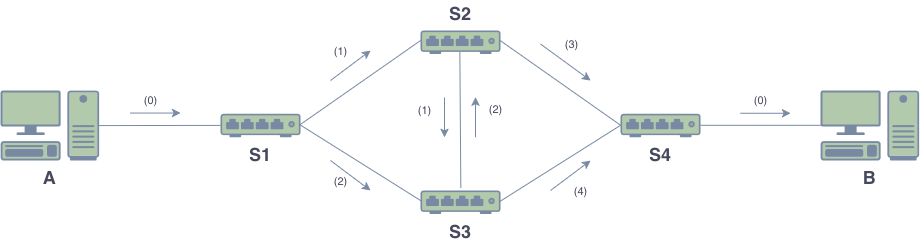
\includegraphics[width=1\textwidth]{img/frer.png}
    \caption{Flusso da host A ad host B mediante switch S1-S4}
    \label{fig:frer}
\end{figure}

In figura \ref{fig:frer} è mostrato un esempio di utilizzo di FRER, in cui il flusso da A a B viene replicato in S1 dove SRF assegna gli ID di sequenza ad i \textit{member stream}, i frame vengono inviati su due percorsi diversi, e successivamente eliminati in S4 tramite IRF mediante un algoritmo a scelta tra MAR o VRA.

\subsection{PCR - Path Control and Reservation}
IEEE 802.1Qca si basa sull'estensione del protocollo IS-IS - \textit{Intermediate System to Intermediate System} \cite{isis}, permette un controllo esplicito del percorso, a differenza di protocolli tradizionali che si basano sul percorso più breve, la possibilità di allocare porzioni di banda e riservare risorse lungo percorsi selezionati e inoltre di gestire la ridondanza e la resilienza dei nodi.
\subsection{PSFP - Per-Stream Filtering and Policing }
IEEE 802.1Qci definisce protocolli e procedure volti a proteggere le reti filtrando, limitando e programmando i dati in ingresso a livello del singolo flusso \cite{8021Qci}.
\section{Gestione risorse e rete}
Il controllo della rete e la gestione delle risorse sono aspetti cruciali per garantire l'allocazione efficiente della banda, la priorità del traffico e il rispetto dei requisiti di QoS - \textit{Quality of Service}.
Per gestire le prenotazioni dei flussi e configurare la rete, gli standard TSN (in particolare IEEE 802.1Qcc, che estende lo Stream Reservation Protocol) definiscono tre opzioni o modelli architetturali principali  \cite{architetture}.
\subsection{Modello Completamente Distribuito}
In questo modello non vi è alcuna entità di gestione centrale. Come è possibile osservare in \ref{fig:full_dist} la rete viene configurata in modo completamente distribuito: i dispositivi finali (Talker e Listener) e i bridge (switch TSN) negoziano direttamente tra loro la registrazione e la prenotazione delle risorse (code, buffer, banda) scambiandosi U/NCI - \textit{User-to-Network Configuration Information}, che viaggia in modalità \textit{hop-by-hop} tra i nodi della rete.
In questo modello il compito della UNI - \textit{User-Network Interface} è quello di agire come confine tra dispositivo finale e bridge.


\begin{figure}[H]
    \centering
    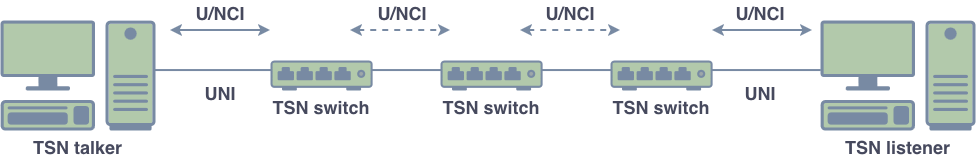
\includegraphics[width=1 \textwidth]{img/fully_distribuited.png}
    \caption{Modello Completamente Distribuito}
    \label{fig:full_dist}
\end{figure}


\subsection{Modello a Rete Centralizzata e Utente Distribuito}
In questo modello, come mostrato in figura \ref{fig:half_cent}, i dispositivi finali inviano le loro specifiche esigenze di rete ai bridge di confine tramite l'interfaccia UNI. La rete, a questo punto, utilizza un'entità centrale chiamata CNC - \textit{Centralized Network Configuration} che riceve questi requisiti e si occupa di configurare tutti i bridge della rete per soddisfare le specifiche.

\begin{figure}[H]
    \centering
    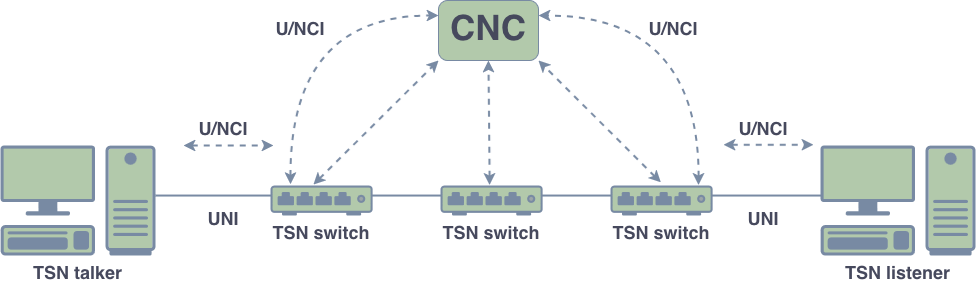
\includegraphics[width=1 \textwidth]{img/half_cetralized.png}
    \caption{Modello a Rete Centralizzata e Utente Distribuito}
    \label{fig:half_cent}
\end{figure}


\subsection{Modello Completamente Centralizzato}
Questo è il modello più avanzato per reti complesse, è possibile notare in figura \ref{fig:full_cent} come qui vengano affiancate due entità software centralizzate:
\begin{itemize}
    \item \textbf{CUC - Centralized User Configuration:} È un'applicazione che funge da proxy per i dispositivi finali. Comunica con essi, raccoglie i requisiti di comunicazione deterministica di cui hanno bisogno e formula una richiesta unica da passare al CNC
    \item \textbf{CNC - Centralized Network Configuration:} Riceve le richieste dal CUC, ha una visione globale della rete e svolge due compiti fondamentali: calcola i percorsi fisici (routing) e le schedulazioni end-to-end per ogni flusso, e infine applica queste configurazioni all'interno dei bridge TSN
\end{itemize}

\begin{figure}[H]
    \centering
    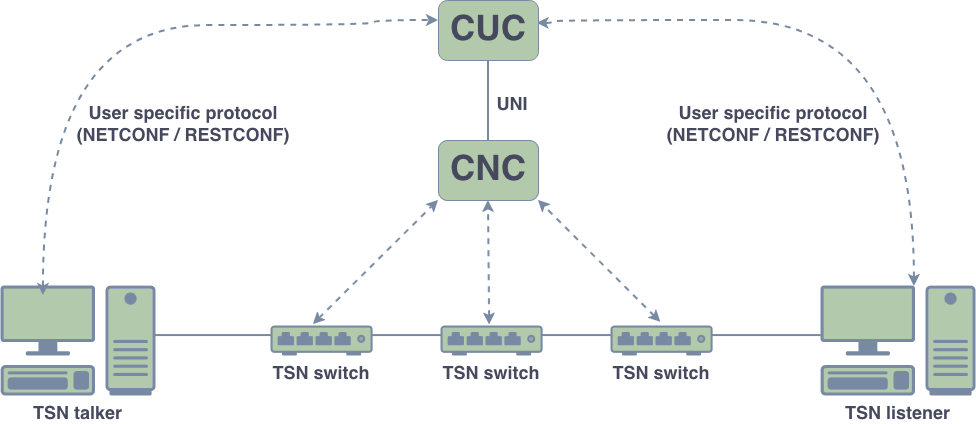
\includegraphics[width=1 \textwidth]{img/fully_centralized.png}
    \caption{Modello Completamente Centralizzato}
    \label{fig:full_cent}
\end{figure}


\subsection{Allocazione delle risorse}
L'ecosistema TSN si avvale di una suite di standard specifici per modellare e allocare le risorse
\begin{itemize}
    \item \textbf{IEEE 802.1Qcp - Modello Dati YANG:} È il cuore della standardizzazione. Fornisce un linguaggio di modellazione unificato (YANG) per descrivere i dati di configurazione, lo stato dei dispositivi e le operazioni. Utilizzando protocolli di gestione di rete sicuri come NETCONF o RESTCONF ,i controller possono inviare queste configurazioni standardizzate a dispositivi di produttori diversi, eliminando il "vendor lock-in"
    \item \textbf{IEEE 802.1CS - Link-Local Registration Protocol:} Ottimizza la replica dei database di registrazione a livello locale (da un capo all'altro di un singolo collegamento). Rispetto ai vecchi protocolli, LRP è in grado di gestire database molto più ampi (nell'ordine di 1 Mbyte), rendendo la gestione distribuita molto più efficiente
    \item \textbf{IEEE P802.1Qdd - Resource Allocation Protocol:} Sfrutta LRP per supportare la prenotazione dinamica delle risorse (per flussi unicast e multicast) all'interno del modello Completamente Distribuito. È nato per superare i limiti di scalabilità del vecchio protocollo MSRP 
    \item \textbf{IEEE P802.1Qdj}: Uno standard in via di sviluppo che mira a chiarire e definire in modo preciso le funzioni specifiche delle due entità centrali, CUC e CNC, e a potenziare l'interfaccia di comunicazione UNI tra di esse
\end{itemize}
Attualmente, la ricerca e l'industria si concentrano fortemente sul modello completamente centralizzato, poiché si sposa perfettamente con i concetti del Software Defined Networking. In questo approccio, concetti come il TSSDN - \textit{Time-Sensitive Software Defined Network} utilizzano un controller SDN per fungere da CNC, separando nettamente il piano dati da quello di controllo \cite{tsn_sdn}.
\\
Il flusso di lavoro operativo si articola in quattro fasi principali:
\begin{enumerate}
    \item \emph{Scoperta della Topologia}: Il CNC esplora la rete utilizzando protocolli come LLDP (Link Layer Discovery Protocol) per ottenere una visione globale di tutti i nodi, i collegamenti e le risorse disponibili
    \item \emph{Richiesta dell'Utente}: I dispositivi finali (Talker/Listener) inviano le loro richieste di servizio al CUC tramite protocolli specifici dell'utente (come OPC UA). Il CUC aggrega queste richieste e le inoltra al CNC attraverso l'interfaccia UNI
    \item \emph{Configurazione della Rete}: Il CNC riceve le richieste, calcola i percorsi di routing ottimali e le schedulazioni temporali complesse (come le Gate Control List per lo standard 802.1Qbv). Converte poi questi calcoli in "profili" YANG e li distribuisce agli switch fisici tramite NETCONF. Infine, conferma l'avvenuta allocazione al CUC
    \item \emph{Monitoraggio e Ripristino}: La rete viene costantemente monitorata. Se si verifica un guasto, i nodi adiacenti lo segnalano al CNC, che ricalcola istantaneamente le rotte e invia nuove configurazioni per isolare o aggirare il problema
\end{enumerate}
\section{WiFi 7}
Obiettivo di questa sezione è descrivere le funzionalità introdotte in 802.11be e come esse risultano fondamentali per permettere lo sviluppo di infrastrutture di comunicazioni deterministiche su reti wireless, per un introduzione allo standard 802.11 si veda \cite{80211overview}.
Le caratteristiche principali introdotte in 802.11be sono:
\begin{itemize}
    \item \textbf{Banda a 320 MHz}
    \item \textbf{MRU -  Multiple Resource Unit}: A partire da 802.11ax - Wifi 6 viene utilizzato OFDMA per dividere un canale in diverse RU - \textit{Resource Unit}, ovvero un blocco di sottoportanti assegnato ad una data stazione, in 802.11be viene introdotta la possibilità di assegnare ad una stessa stazione per uno stesso  PPDU - \textit{Physical Layer Protocol Data Unit} più RU.
    Oltre ad incrementare il throughput e l'efficienza ciò permette di effettuare il \textit{preamble puncturing}, ovvero indicare in un campo specifico del frame che uno o più canali del RU sono "forati", così facendo il ricevente eviterà di demodulare quella specifica frequenza.
    \\
    Questo problema nasce dal fatto che alcune porzioni di frequenza 5GHz sono condivise con radar militari/meteorologici. Per maggiori informazioni si veda \cite{wifi7_punc}

    \begin{figure}[H]
    \centering
    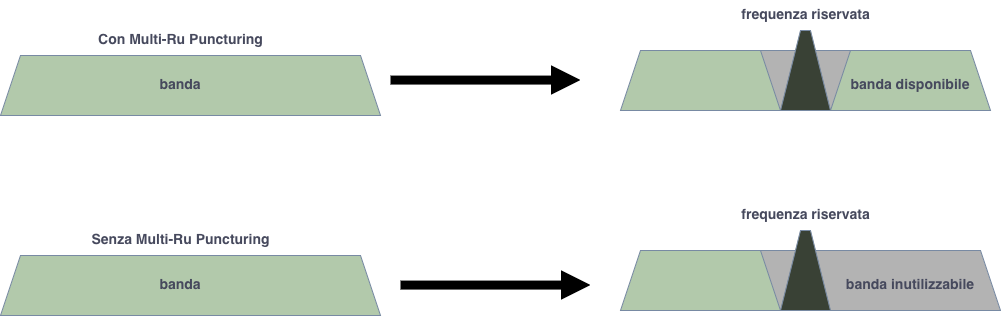
\includegraphics[width=1 \textwidth]{img/preamble_puncturing.png}
    \caption{Effetti del preamble puncturing nella gestione della banda}
    \label{fig:preample_punct}
    \end{figure}

    In figura \ref{fig:preample_punct} è mostrata la differenza tra un frame senza \textit{preamble puncturing}, in cui il canale a causa di una frequenza riservata perde la possibilità di utilizzare una porzione di banda disponibile, ed il caso con \textit{preamble puncturing}, dove è possibile osservare come una porzione minima, ed equivalente alla frequenza inutilizzabile del canale, è "forata" e non viene quindi utilizzata per la trasmissione.

    \item \textbf{Modulazione 4096 QAM}: Si ha un miglioramento del 20\% rispetto a WiFi 6/6E
    \item \textbf{1024 A-MDPU}: Aggregate MAC Protocol Data Unit introdotto inizialmente nel 802.11n permette di aggregare più MPDU in unico frame, a cui viene assegnato un solo header del livello fisico, questo e il fatto che il ricevente manderà un solo block acknowledgment permette di sfruttare in maniera più efficiente il canale radio e di diminuire il tempo di contesa del canale, 802.11be permette di aggregare fino a 1024 MPDU
    \item \textbf{MLO - Multi-Link Operation}: Permette ad una stazione di utilizzare più interfacce radio contemporaneamente, anche su bande diverse, per trasmettere e ricevere dati. Ciò consente di aumentare la capacità complessiva, ridurre la latenza e migliorare l'affidabilità, poiché se un link è congestionato o ha interferenze, la stazione può continuare a comunicare attraverso gli altri link disponibili.
    \\
    Una delle principali innovazioni apportate in 802.11be, permette alle stazioni e agli access-point di trasmettere e ricevere dati appartenenti allo stesso flusso di traffico attraverso diverse interfacce radio.
    Vengono definiti MLD - \textit{Multi-Link Device} sia gli access point che le stazioni dotati di molteplici interfacce radio, i quali, dopo aver stabilito un'unica connessione possono comunicare contemporaneamente su più bande.
    \\
    In figura \ref{fig:mlo} è mostrato un esempio di MLO, in cui 2 MLD, una stazione e un access point entrambi dotati di tre interafacce radio,
    comunicano sui diversi link.
    \\
    Si ha un unico indirizzo MAC per MLD ma nonostante questo, i link sono indipendenti (ognuno gestisce il proprio CSMA/CA, back-off e NAV).
    Le modalità di utilizzo possibile definite dallo standard sono
    \begin{enumerate}
        \item \textbf{STR - Simultaneous Transmit e Receive}: Il dispositivo MLD trasmette e riceve in parallelo su link diversi, massima efficienza ma costo computazionale e consumi elevati
        \item \textbf{NSTR - Non-Simultaneous Transmit e Receive}: Se i link sono troppo vicini la trasmissione e la ricezione contemporanea potrebbe creare delle interferenze in-device, in questo modalità non è possibile inviare e ricevere contemporaneamente, ma solo inviare o ricevere.
        \item \textbf{eMLSR - Enhanced Multi-Link Single Radio}: Introdotta per dispositivi a basso consumo, utilizza un solo canale radio e si sposta dinamicamente tra i link a seconda del traffico. \cite{str_emlsr}
    \end{enumerate}
    \begin{figure}[H]
    \centering
    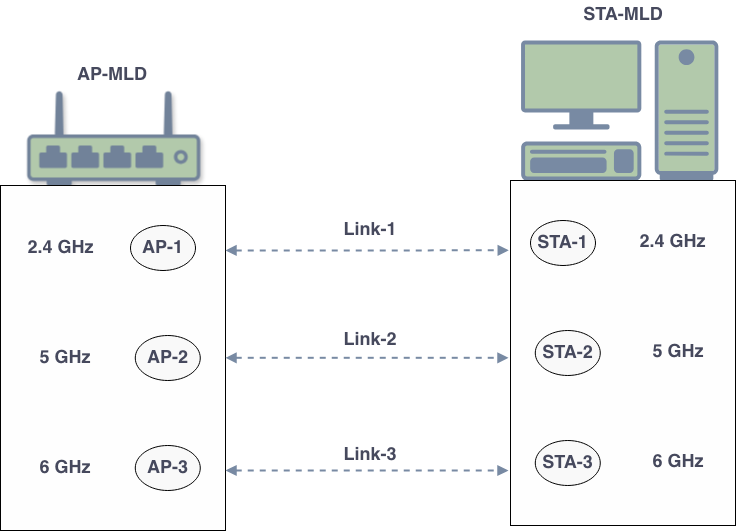
\includegraphics[width=1 \textwidth]{img/mlo.png}
    \caption{Diagramma MLO}
    \label{fig:mlo}
    \end{figure}
    \item \textbf{R-TWT - Restricted Target Wake Time}: È l'evoluzione dei meccanismi di risparmio energetico nei dispositivi wireless, PSM e TWT, introdotto in 802.11be estende la possibilità di negoziare i SP - \textit{Service Period} e WI - \textit{Wake Interval} già presente in TWT, supportando accesso esclusivo al canale di comunicazione durante il SP a determinate STA o TID - \textit{Traffic IDentifier}. Questo meccanismo implica quindi una determinata QoS e si avvicina a ciò che abbiamo già visto con lo standard 802.1Qbv, per più dettagli su R-TWT si veda \cite{rtwt}
\end{itemize}
\subsection{Supporto al TSN}
Le reti wireless hanno storicamente operato secondo il paradigma \textit{best-effort}: il mezzo condiviso, l'accesso probabilistico CSMA/CA e il fading radio rendevano impossibile garantire latenza bounded o affidabilità deterministica. Questa limitazione ha confinato Wi-Fi a scenari \textit{consumer}, escludendolo dagli ambiti industriali, medicali e di controllo in tempo reale, dove IEEE 802.1 TSN stava invece diventando lo standard di riferimento per le reti cablate. 
\\
Wi-Fi 7 nasce esplicitamente per rispondere a questo obiettivo: comunicazioni EHT - \textit{Extremely High Throughput} combinate con latenza deterministica e ultra-reliability, colmando il gap tra Wi-Fi e TSN.
\\
È possibile trovare lavori in letteratura \cite{wifi7tsn}, dove viene sottolineata la possibilità di mappare il protocollo 802.1CB su 802.11be grazie all'introduzione del MLO.


\chapter{Stack 802.11 in Linux e supporto al TSN}
\section{Stack 802.11}
Originariamente, la gestione del wireless in Linux era affidata alle WEXT - \textit{Wireless Extensions}. Sebbene funzionali per i primi standard (802.11b/g), le WEXT  presentavano limitazioni strutturali, come l'uso di \texttt{ioctl} e l'incapacità di scalare verso configurazioni multi-interfaccia complesse.
Ad oggi per fornire un canale di comunicazione bidirezione tra lo \textit{userspace} e il \textit{kernelspace} sono disponibili le Netlink socket, un meccanismo nato come estensione delle socket standard per supportare IPC. 
\\
Per un approfondimento sul perchè il passaggio alle socket Netlink sia stato necessario si veda \cite{netlink}.
\\
L'architettura moderna mostrata in figura \ref{fig:80211linuxstack}, che andremo a considerare d'ora in poi, si basa su una struttura composta da molteplici moduli kernel i quali implementano le due seguenti funzionalità:
\begin{itemize}
    \item \textbf{SME - Station Management Entity}: È l'entità logica di gestione di più alto livello all'interno di una stazione 802.11. Opera al di sopra del MAC layer e ha la responsabilità di prendere decisioni di policy: quali reti scansionare, quando associarsi, quando rieseguire l'autenticazione, quando cambiare canale
    \item \textbf{MLME - MAC Layer Management Entity}: È l'entità di gestione del sottostrato MAC. Se la SME decide cosa fare, la MLME esegue tali decisioni a livello MAC, generando e interpretando i frame di gestione 802.11 (Probe Request/Response, Authentication, Association, Deauthentication, ecc.).
\end{itemize}

\begin{figure}[H]
    \centering
    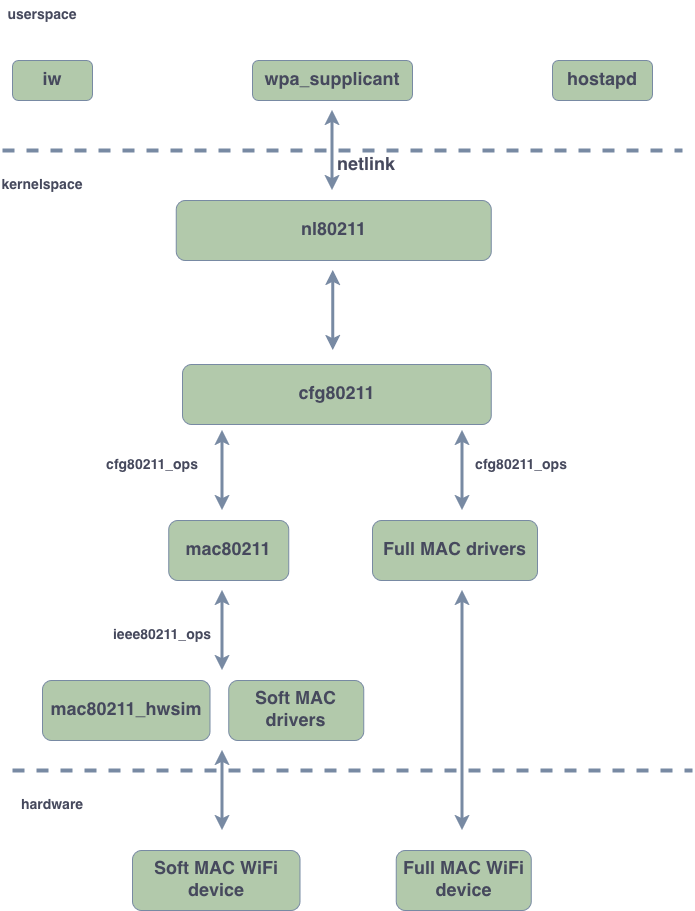
\includegraphics[width=0.8\textwidth]{img/linuxstack.png}
    \caption{Stack 802.11 in Linux}
    \label{fig:80211linuxstack}
\end{figure}


I principali moduli kernel che implementano queste funzionalità sono:
\begin{itemize}
    \item \textbf{nl80211}: Costituisce l'interfaccia standard di comunicazione tra le applicazioni in userspace e il sottosistema wireless del kernel. Attraverso di essa, diversi strumenti software possono interrogare, configurare e controllare le interfacce IEEE 802.11 in modo uniforme, senza dipendere direttamente dai dettagli implementativi del driver sottostante. Gli utenti di \texttt{nl80211} sono:
    \begin{itemize}
        \item \textbf{iw}: Utility di configurazione a basso livello che consente di eseguire operazioni puntuali quali la scansione delle reti disponibili, la lettura delle capacità del dispositivo e la modifica dei parametri dell'interfaccia
        \item \textbf{wpa\_supplicant e hostapd}: Impiegati rispettivamente per la gestione di una stazione client e di un access point
        \item \textbf{crda}: Dedicato alla gestione del dominio regolatorio
        \item \textbf{iwd}: Demone per la gestione delle connessioni Wi-Fi
        \item \textbf{NetworkManager}: Realizza alcune funzioni di discovery
    \end{itemize}
    \item \textbf{cfg80211}: Rappresenta il sottosistema di configurazione centrale per 802.11 in Linux fornendo un'astrazione unificata dei dispositivi wireless: \texttt{wiphy} 
    \item \textbf{mac80211}: È il framework di gestione del livello MAC per i dispositivi definiti SoftMAC.
    \\
    In un'architettura SoftMAC il dispositivo fisico si occupa solamente del livello fisico, mentre la gestione del protocollo è demandata al processore tramite appunto il modulo kernel \texttt{mac80211}
    \\
    Invece in un'architettura FullMAC, i dispositivi integrano la logica MLME direttamente nel firmware del dispositvo. La scheda di rete appare al sistema operativo come un'entità autonoma che gestisce internamente la complessità del protocollo 802.11.
    \item \textbf{mac80211\_hwsim}: Nel contesto dello stack wireless Linux, \texttt{mac80211\_hwsim} è un modulo del kernel che consente di emulare una o più radio IEEE 802.11 interamente mediante software, senza richiedere hardware fisico dedicato.
    \\ 
    Dal punto di vista architetturale, \texttt{mac80211\_hwsim} sostituisce il livello radio fisico con un meccanismo software che simula la trasmissione dei frame tra interfacce virtuali, mantenendo invariati i livelli superiori dello stack, in particolare \texttt{mac80211}, \texttt{cfg80211} e \texttt{nl80211}. 
    \\
    Di conseguenza, applicazioni come \texttt{iw}, \texttt{wpa\_supplicant} e \texttt{hostapd} possono essere impiegate senza modifiche anche in ambienti emulati, poiché l'interazione con il sottosistema wireless del kernel avviene secondo le stesse primitive previste per l'hardware reale. 
    \\
    Questa proprietà rende \texttt{mac80211\_hwsim} particolarmente utile in attività di sviluppo, testing e ricerca, dove è importante disporre di scenari wireless controllati, riproducibili e facilmente osservabili. 
\end{itemize}

\section{Mappare servizi TSN in Linux}
Obiettivo di questa sezione è quello di, partendo dagli obiettivi principali del TSN visti in maniera approfondita nel capitolo \ref{chap:cap1} capire come essi possono essere garantiti in Linux.

\subsection{Sincronizzazione temporale: Linux PTP}
Linux PTP - \textit{Precision Time Protocol} è una suite di software nata per implementare lo standard IEEE 1588, su cui è a sua volta basato lo standard 802.1AS. Fornisce due strumenti principali:
\begin{itemize}
    \item \textbf{ptp4l}: È il demone che implementa a tutti gli effetti il protocollo PTP ed è responsabile della coordinazione e sincronizzazione temporale tra dispositivi
    \item \textbf{phc2sys}: È il demone che sincronizza il PHC, ovvero l'orologio hardware integrato nelle NIC IEEE 1588 compliant, con l'orologio del sistema al fine di garantire consistenza
\end{itemize}

\subsubsection{Gerarchie}
Linux PTP sfrutta una struttura gerarchica per delineare diversi tipi di dispositivi all'interno del dominio PTP:
\begin{itemize}
    \item \textbf{GM - Grand Master Clock}: È l'orologio di riferimento, scelto mediante algoritmo BMCA - \textit{Best Master Clock Algorithm}, 
    rappresenta la sorgente temporale di riferimento per il dominio PTP 
    \item \textbf{OC - Ordinary Clock}: È un qualsiasi dispositivo dotato di una singola porta, che si comporta o da master o da slave
    \item \textbf{BC - Boundary Clock}: È un dispositivo dotato di più porte, su una porta, esso si sincronizza rispetto ad un master, e sulle altre porte assume il ruolo di master alla quale degli slave si sincronizzeranno
    \item \textbf{TC - Transparent Clock}: È un dispositivo che ha solo il compito di inoltrare un messaggio PTP, ha il compito di compensare il tempo in cui il messaggio ha passato sul dispositivo di inoltro
\end{itemize}
\subsubsection{Modalità PTP e Scambio di messaggi}
Linux PTP supporta due modalità di sincronizzazione:
\begin{enumerate}
    \item \textbf{One-step mode}: I timestamp sono inclusi nei messaggi di \texttt{Sync}
    \item \textbf{Two-step mode}: I timestamp sono inviati separatamente in dei messaggi di \texttt{Follow\_Up} per una maggiore accuratezza
\end{enumerate}
Il processo di sincronizzazione, mostrato in figura \ref{fig:linuxptp}, prevede cinque tipi principali di messaggi:
\begin{enumerate}
    \item \textbf{Announce Message}: Inviato da OC e BC ha lo scopo di pubblicizzare le caratteristiche del proprio orologio e partecipare al processo di selezione del BCMA
    \item \textbf{Sync Message}: Inviato dal GM trasmette il tempo attuale agli slave per avviare sincronizzazione
    \item \textbf{Follow\_Up}: Inviato dal GM agli slave in modalità two-step, contiene il timestamp di invio del messaggio \texttt{Sync}
    \item \textbf{Delay\_Req}: Inviato dagli slave al GM per misurare il ritardo di propagazione
    \item \textbf{Delay\_Resp}: Inviato dal GM agli slave in risposta a \texttt{Delay\_Req}, contiene il timestamp di ricezione del messaggio  \texttt{Delay\_Req}
\end{enumerate}

\begin{figure}[H]
    \centering
    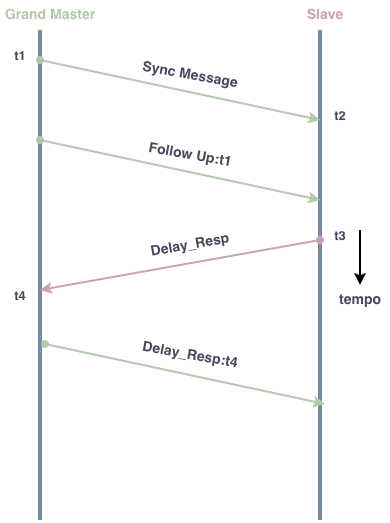
\includegraphics[width=0.5\textwidth]{img/ptp.png}
    \caption{Processo di sincronizzazione two-step mode}
    \label{fig:linuxptp}
\end{figure}
In figura \ref{fig:linuxptp} è mostrato un esempio di processo di sincronizzazione in modalità two-step, in cui il GM invia un messaggio \texttt{Sync} agli slave, successivamente invia un messaggio \texttt{Follow\_Up} contenente il timestamp di invio del messaggio \texttt{Sync}, gli slave a questo punto possono calcolare la differenza tra il tempo del GM e il proprio tempo locale, e inviare un messaggio \texttt{Delay\_Req} al GM per misurare il ritardo di propagazione, infine il GM risponde con un messaggio \texttt{Delay\_Resp} contenente il timestamp di ricezione del messaggio \texttt{Delay\_Req}, permettendo agli slave di compensare il ritardo di propagazione e sincronizzarsi con il GM.
Per informazioni piu dettagliate e istruzioni sull'installazione di Linux PTP si veda \cite{linux_ptp}.
\subsubsection{Esempio di configurazione e utilizzo Linux PTP}
\label{section:esempio_ptp}
Per mostrare come è possibile utilizzare e configurare Linux PTP verranno utizzati tre container Docker, \texttt{node1} e \texttt{node2} con il ruolo di OC e \texttt{node3} con il ruolo di GM, in appendice \ref{Appendice:docker_ptp} è riportato lo script bash utilizzato per la configurazione.

Le tre macchine virtuali sono collegate tra loro tramite un bridge Docker, e sono dotate di una scheda di rete virtuale che supporta PTP solamente tramite timestamping software con conseguenze evidenti sulle prestazioni.

Configuriamo le due macchine \texttt{node1} e \texttt{node2}, che svolgeranno il ruolo di OC, con il seguente file di configurazione per \texttt{ptp4l}

\begin{lstlisting}[
    basicstyle=\ttfamily\small,
    breaklines=true,
    breakatwhitespace=true,
    frame=single,
    numberstyle=\tiny,
    caption={Esempio di configurazione PTP per OC (/etc/ptp4l.conf)},
    label={code:ptp_oc_conf}
]
    [global]
    priority1               128 # Primo criterio di elezione del master
    priority2               128 # Secondo criterio di elezione del master per tie-break
    clockClass              135 # Descrive la qualita della sorgente di tempo del clock
    clockAccuracy           0xFE # Descrive la precisione del clock (0xFE indica sconosciuta)
    offsetScaledLogVariance 0xFFFF # Descrive la varianza scalata del clock (0xFFFF indica sconosciuta)
    domainNumber            0 # Numero di dominio PTP (0-255)
    logAnnounceInterval     1 # Intervallo dei messaggi di annuncio 
    logSyncInterval         0 # Intervallo dei messaggi di sincronizzazione 
    logMinDelayReqInterval  0 # Intervallo minimo di richiesta di ritardo 
    announceReceiptTimeout  3 # Intervallo prima che la porta dichiari il master assente
    dataset_comparison      ieee1588 # Algoritmo usato per il confronto nel BMCA
\end{lstlisting}



Configuraiamo invece  \texttt{node3} con il ruolo di GM nel seguente modo:

\begin{lstlisting}[
    basicstyle=\ttfamily\small,
    breaklines=true,
    breakatwhitespace=true,
    frame=single,
    numberstyle=\tiny,
    caption={Esempio di configurazione PTP per GM (/etc/ptp4l.conf)},
    label={code:ptp_gm_conf}
]
    [global]
    priority1               127
    priority2               128
    clockClass              135
    clockAccuracy           0xFE
    offsetScaledLogVariance 0xFFFF
    domainNumber            0
    logAnnounceInterval     1
    logSyncInterval         0
    logMinDelayReqInterval  0
    announceReceiptTimeout  3
    dataset_comparison      ieee1588
\end{lstlisting}

Possiamo notare che la configurazione è molto simile, l'unica differenza è il valore di \texttt{priority1}, che è più basso per il GM, in questo modo, durante il processo di elezione del master, \texttt{node3} sarà preferito rispetto a \texttt{node1} e \texttt{node2}.

Una volta scritti i file di configurazione, è possibile avviare il servizio eseguendo il comando \texttt{ptp4l -i eth0 -f /etc/ptp4l.conf -S -m -q} dove:
\begin{itemize}
    \item \texttt{-i eth0}: Specifica l'interfaccia di rete da utilizzare per la sincronizzazione
    \item \texttt{-f /etc/ptp4l.conf}: Specifica il file di configurazione da utilizzare
    \item \texttt{-S}: Abilita la modalità di timestamping software
    \item \texttt{-m}: Abilita la stampa dei messaggi su stdout
    \item \texttt{-q}: Disablita logging su syslog
\end{itemize}

Osservando output di \texttt{ptp4l} su \texttt{node3} in \ref{code:node3_ptp} è possibile notare che esso assume il ruolo di GM, mentre \texttt{node1} e \texttt{node2} assumono il ruolo di slave e avviano il processo di sincronizzazione come è possibile osservare \ref{code:node1_ptp} (viene mostrato un singolo output in quanto analoghi).

\begin{lstlisting}[
    basicstyle=\ttfamily\small,
    breaklines=true,
    breakatwhitespace=true,
    frame=single,
    numberstyle=\tiny,
    caption={Stdout node3 - processo di elezione del master},
    label={code:node3_ptp}
]
    3fb1aacceb52:/# ptp4l -i eth0 -f /etc/ptp4l.conf -S -m -q
    ptp4l[5314.111]: port 1 (eth0): INITIALIZING to LISTENING on INIT_COMPLETE
    ptp4l[5314.114]: port 0 (/var/run/ptp4l): INITIALIZING to LISTENING on INIT_COMPLETE
    ptp4l[5314.114]: port 0 (/var/run/ptp4lro): INITIALIZING to LISTENING on INIT_COMPLETE
    ptp4l[5320.303]: port 1 (eth0): new foreign master c6b50d.fffe.d8e020-1
    ptp4l[5320.397]: port 1 (eth0): new foreign master 3aa0ac.fffe.2a0af2-1
    ptp4l[5321.213]: port 1 (eth0): LISTENING to MASTER on ANNOUNCE_RECEIPT_TIMEOUT_EXPIRES
    ptp4l[5321.213]: selected local clock a6945b.fffe.0a2fb2 as best master
    ptp4l[5321.213]: port 1 (eth0): assuming the grand master role
\end{lstlisting}

\vspace{2.5cm}

\begin{lstlisting}[
    basicstyle=\ttfamily\small,
    breaklines=true,
    breakatwhitespace=true,
    frame=single,
    numberstyle=\tiny,
    caption={Stdout node1 - processo di elezione del master e sincronizzazione},
    label={code:node1_ptp}
]
    c5a775638645:/# ptp4l -i eth0 -f /etc/ptp4l.conf -S -m -q
    ptp4l[5312.811]: port 1 (eth0): INITIALIZING to LISTENING on INIT_COMPLETE
    ptp4l[5312.813]: port 0 (/var/run/ptp4l): INITIALIZING to LISTENING on INIT_COMPLETE
    ptp4l[5312.813]: port 0 (/var/run/ptp4lro): INITIALIZING to LISTENING on INIT_COMPLETE
    ptp4l[5320.298]: port 1 (eth0): LISTENING to MASTER on ANNOUNCE_RECEIPT_TIMEOUT_EXPIRES
    ptp4l[5320.299]: selected local clock c6b50d.fffe.d8e020 as best master
    ptp4l[5320.299]: port 1 (eth0): assuming the slave role
    ptp4l[5324.408]: port 1 (eth0): MASTER to UNCALIBRATED on RS_SLAVE
    ptp4l[5325.222]: selected best master clock a6945b.fffe.0a2fb2
    ptp4l[5325.222]: foreign master not using PTP timescale
    ptp4l[5327.237]: master offset     -44063 s0 freq   -1563 path delay     90896
    ptp4l[5328.238]: master offset      12729 s0 freq   -1563 path delay     90896
    ptp4l[5329.239]: master offset     -56051 s0 freq   -1563 path delay     88968
    ptp4l[5330.244]: master offset      19991 s0 freq   -1563 path delay     67801
    ptp4l[5343.277]: master offset     -35019 s1 freq   -1000 path delay     54603
    ptp4l[5344.278]: clockcheck: clock frequency changed unexpectedly!
    ptp4l[5344.278]: master offset       9105 s2 freq     -80 path delay     54603
    ptp4l[5344.278]: port 1 (eth0): UNCALIBRATED to SLAVE on MASTER_CLOCK_SELECTED
    ptp4l[5345.280]: master offset     -37187 s2 freq   -4746 path delay     54062
    ptp4l[5346.283]: clockcheck: clock frequency changed unexpectedly!
\end{lstlisting}

Nell'output di \texttt{node1} mostrato in \ref{code:node1_ptp} è possibile osservare che esso assume il ruolo di slave, e poi la successione di tre fasi principali del processo di sincronizzazione:
\begin{itemize}
    \item \textbf{s0}: Fase iniziale in cui lo \textit{slave} ha appena iniziato a ricevere messaggi dal \textit{master}, ma non ha ancora abbastanza informazioni per calcolare un offset accurato quindi non effettua operazioni di correzione del clock
    \item \textbf{s1}: Fase in cui \texttt{ptp4l} invoca una primitiva di sistema per spostare il clock locale esattamente al tempo del \textit{master}, in questo modo si ha un salto temporale che può essere significativo, ma permette di avvicinare lo slave al master, non avviene sempre, ma solo quando l'offset è superiore ad una certa soglia chiamata \textit{first\_step\_threshold}
    \item \textbf{s2}: Fase in cui il protocollo va a regime e lo \textit{slave} corregge continuamente il proprio clock
\end{itemize}
\section{Latenza Limitata e 802.1Q: VLAN, TAPRIO, Frame Preemption}
Come analizzato nel Capitolo \ref{chap:cap1}, i protocolli e i meccanismi per garantire una latenza limitata e azzerare le perdite causate dalla congestione sono diversi, ma tutti basati sul protocollo 802.1Q, Bridges e Bridges Networks, dove abbiamo visto è centrale il ruolo delle VLAN.
\\
In Linux \texttt{iproute2} è un insieme di strumenti a riga di comando per la gestione del networking, basato su Netlink socket per l'interazione con lo stack di rete del kernel, tra le sue diverse funzionalità è presente il supporto alla creazione e gestione di VLAN, per maggiori informazioni si veda \cite{vlan_linux} e \cite{vlan_linux_setup_iproute2}.
\\
\subsection{tc}
Tra le diverse funzionalità di \texttt{iproute2} è presente anche \texttt{tc} - \textit{Traffic Control}, che ci permette di configurare lo scheduler dei pacchetti kernel, i pilastri di \texttt{tc} sono:
\begin{itemize}
    \item \textbf{qdisc - Queueing Discipline}: È la disciplina di accodamento, ovvero l'algoritmo che decide quale pacchetto trasmettere, è possibile configurare più \texttt{qdisc} in cascata, ad esempio, è possibile utilizzare un \texttt{qdisc} per implementare una coda per ogni classe di traffico e un secondo \texttt{qdisc} per implementare l'algoritmo di accodamento
    \item \textbf{class}: Rappresenta una classe di traffico, è possibile configurare più classi di traffico, ad esempio, una per il traffico critico e una per il traffico best-effort
    \item \textbf{filter}: Permette di classificare i pacchetti in ingresso, ad esempio, è possibile configurare un filtro per classificare i pacchetti in base al campo PCP del frame 802.1Q
\end{itemize}
Ad oggi i \texttt{qdisc} offerti da Linux che supportano TSN sono:
\begin{itemize}
    \item \textbf{taprio}: Implementa l'algoritmo TAS, permette di configurare le GCL per ogni classe di traffico
    \item \textbf{cbs}: Implementa l'algoritmo CBS, permette di configurare i parametri di credito per ogni classe di traffico
    \item \textbf{etf}: Implementa il meccanismo di invio basato sul tempo (TxTime), permettendo di trasmettere i pacchetti a intervalli temporali precisi e predefiniti, garantendo il determinismo nei sistemi real-time
\end{itemize}
Per maggiori informazioni riguardo gli algoritmi e le loro implementazioni si faccia riferimento alla documentazione ufficiale \cite{tsn_qdiscs}.
\\
\subsubsection{Esempio di configurazione taprio tramite tc}
In figura \ref{code:tc_taprio} è riportato un comando per configurare tramite \texttt{tc} una \texttt{qdisc} che implementa \texttt{taprio}:
\begin{lstlisting}[
    basicstyle=\ttfamily\small,
    breaklines=true,
    breakatwhitespace=true,
    frame=single,
    numberstyle=\tiny,
    caption={Esempio di configurazione di taprio con tc},
    label={code:tc_taprio}
]
    tc qdisc add dev eth0 \
        parent root handle 100: \
        taprio \
        num_tc 3 \
        map 2 2 2 2 1 1 0 0 \
        queues 1@0 1@1 1@2 \
        base-time 1000000000 \
        sched-entry S 01 200000 \
        sched-entry S 02 300000 \
        sched-entry S 04 500000 \
        flags 0x0 \
        clockid CLOCK_TAI
\end{lstlisting}

I campi principali sono:
\begin{itemize}
    \item \texttt{num\_tc}: Numero di classi di traffico, in questo caso 3, una per il traffico critico, una per il traffico \textit{time sensitive} e una per il traffico \textit{best-effort}
    \item \texttt{map}: Mappa le classi di traffico appena definite ad una priority (0-7), in questo caso la classe 0 è la più prioritaria associata ai livelli 6 e 7, seguita dalla classe 1 associata ai livelli 4 e 5, e infine dalla classe 2 associata ai livelli 0 e 3. Successivamente la priorità verrà estratta dal campo PCP del frame 802.1Q per classificare i pacchetti in ingresso, o dall'opzione \texttt{SO\_PRIORITY} della socket.
    \item \texttt{queues}: Associa le code hardware alle code tc seguendo il formato \texttt{numero\_code@indice\_coda}, in questo caso abbiamo 3 code hardware associate alle 3 classi di traffico, potremmo però avere più code hardware, il che che ci permetterebbe di associarne di più alla classe di traffico critica
    \item \texttt{sched-entry}: Ogni riga definisce uno slot della GCL nel formato \texttt{sched-entry S bitmap duration}, dove \texttt{S} indica che si tratta di uno slot statico, \texttt{bitmap} è una bitmap che indica quali classi di traffico possono essere trasmesse durante lo slot, e \texttt{duration} è la durata dello slot in nanosecondi
    \item \texttt{flags}: Modalità operativa di taprio, \texttt{0x0} indica che \texttt{taprio} è in modalità software, dove i gate sono gestiti dal kernel
\end{itemize}

\subsection{Frame Preemption}
In Linux, il supporto alla Frame Preemption è fornito attraverso \texttt{ethtool} e le \texttt{qdisc} \texttt{mqprio} o \texttt{taprio}.
\\
\texttt{ethtool} è l'utility di amministrazione delle interfacce Ethernet e consente di interrogare e configurare alcune funzionalità avanzate del controller di rete, comprese quelle necessarie per abilitare la preemption. Il meccanismo implementa quanto previsto dagli standard IEEE 802.1Qbu e IEEE 802.3br, distinguendo tra traffico critico, che non può essere interrotto, e traffico preemptable, che può essere sospeso temporaneamente per consentire la trasmissione immediata di frame più urgenti.
\\
\\
Dal punto di vista architetturale, la funzionalità si basa sul MAC Merge layer, un sottolivello del MAC che coordina due flussi logici distinti: uno dedicato al traffico express e uno a quello prelazionabile.
\\
Quando necessario, il MAC Merge layer consente di frammentare un frame prelazionabile, inserire il frame critico e riprendere successivamente la trasmissione del traffico interrotto. 
\\
\subsubsection{Esempio di configurazione frame preemption tramite tc}
Per configurare e utilizzare Frame Preemption in Linux è necessario innanzitutto abilitare la funzionalità tramite il comando
\begin{lstlisting}[
    basicstyle=\ttfamily\small,
    breaklines=true,
    breakatwhitespace=true,
    frame=single,
    numberstyle=\tiny,
    caption={Abilitazione della Frame Preemption con ethtool},
    label={code:enable_frame_preemption}
]
    ethtool --set-frame-preemption eth0 \
        fp on \
        min-frag-size 60
\end{lstlisting}

Successivamente sarà necessario configurare una \texttt{qdisc} che supporti la preemption, ad esempio \texttt{mqprio} o \texttt{taprio}, in questo caso mostreremo un esempio di configurazione con \texttt{taprio} in quanto già introdotta in precedenza.
\begin{lstlisting}[
    basicstyle=\ttfamily\small,
    breaklines=true,
    breakatwhitespace=true,
    frame=single,
    numberstyle=\tiny,
    caption={Abilitazione della Frame Preemption con ethtool},
    label={code:enable_frame_preemption}
]
    tc qdisc replace dev eth0 \
        parent root handle 100: taprio \
        num_tc 3 \
        map 2 2 2 2 1 1 0 0 \
        queues 1@0 1@1 1@2 \
        base-time 1000000000 \
        sched-entry S 01 200000 \
        sched-entry S 02 300000 \
        sched-entry S 04 500000 \
        flags 0x2 \
        fp expr expr preemptable \
        clockid CLOCK_TAI0
\end{lstlisting}

La configurazione è analoga a quella mostrata in \ref{code:tc_taprio}, l'unica differenza è il campo \texttt{flags} impostato a \texttt{0x2} per indicare che \texttt{taprio} è in modalità hardware, dove i gate sono gestiti dalla NIC, e la presenza dell'opzione \texttt{fp expr expr preemptable} che assegna alle prime due classi di traffico la possibilità di interrompere la trasmissione di pacchetti appartenenti all'ultima classe definita preemptable.
\\
In \ref{chap:cap1}, si è discusso di come algoritmi di schedulazione del traffico basati su un clock condiviso non siano sempre ideali, per questo veniva introdotto ATS, attualmente non è presente un'implementazione ufficiale dello standard IEEE 802.1Qcr, ma in letteratura sono presenti lavori \cite{ats_linux_tc} che dimostrano che con \texttt{tc} si può approssimare ATS nella variante UBS/TBE, nonostante ciò viene sottolineato che per un'implementazione completa servirebbero nuove primitive o nuove \texttt{qdisc} dedicate nel kernel.

\section{Affidabilità: FRER}
Nel kernel Linux non è attualmente disponibile un'implementazione nativa e completa dello standard IEEE 802.1CB - Frame Replication and Elimination for Reliability comparabile, ad esempio, al supporto offerto per altri meccanismi TSN tramite \texttt{qdisc} dedicate.
\\
Tuttavia, il sistema mette a disposizione strumenti programmabili a basso livello che consentono di realizzarne implementazioni sperimentali. Un esempio rilevante è XDP FRER, che propone una realizzazione parziale del paradigma FRER mediante eBPF/XDP \cite{xdp}. 
\\
In tale approccio, la replicazione dei frame viene effettuata su più interfacce di uscita, mentre sul nodo ricevente una funzione di eliminazione provvede a riconoscere e scartare le copie duplicate, consegnando allo stack superiore un solo pacchetto valido. Sebbene questa soluzione non costituisca un supporto standard integrato nel kernel, essa dimostra che Linux dispone di primitive sufficientemente flessibili per implementare meccanismi di affidabilità per-packet in modo efficiente.

\subsubsection{Esempio utilizzo XDP FRER}
Per mostrare il funzionamento di XDP FRER, faremo riferimento all'ambiente di test fornito dall'autore di \cite{xdp}, in cui viene proposta un'infrastrutta composta da due nodi, un \textit{Transitter} ed un \textit{Listener}, collegati tra loro tramite una serie di switch virtuali.

Per configurare gli switch virtuali in entrambe le direzioni per abilitare la replicazione ed eliminazione dei frame, è possibile utilizzare i seguenti comandi:

\begin{lstlisting}[
    basicstyle=\ttfamily\small,
    breaklines=true,
    breakatwhitespace=true,
    frame=single,
    numberstyle=\tiny,
    caption={Avvio di XDP FRER per replicazione ed eliminazione dei frame},
    label={code:xdpfrer_config}
]
    # transimetter -> listener
        nsx xdpfrer -m repl -i aeth0:10 -e enp3s0:55 -e enp6s0:56
        nsx xdpfrer -m elim -i enp4s0:55 -i enp7s0:56 -e beth0:20

    # listener -> transimetter
        nsx xdpfrer -m repl -i beth0:20 -e enp4s0:66 -e enp7s0:67
        nsx xdpfrer -m elim -i enp3s0:66 -i enp6s0:67 -e aeth0:10
\end{lstlisting}

Dove \texttt{nsx xdpfrer -m repl -i aeth0:10 -e enp3s0:55 -e enp6s0:56} significa che i pacchetti con VLAN ID 10 in ingresso sull'interfaccia \texttt{aeth0} vengono replicati su \texttt{enp3s0} e \texttt{enp6s0} con VLAN ID 55 e 56 rispettivamente.
\\
Mentre \texttt{nsx xdpfrer -m elim -i enp4s0:55 -i enp7s0:56 -e beth0:20} significa che i pacchetti in ingresso su \texttt{enp4s0} con VLAN ID 55 e su \texttt{enp7s0} con VLAN ID 56 vengono processati per l'eliminazione dei duplicati e consegnati su \texttt{beth0} con VLAN ID 20.
\\
Si noti che \texttt{nsx} è l'alias per entrare nel namesapce dello switch FRER, in questa implementazione il VLAN ID si comporta stream ID per identificare a quale flusso appartiene un frame e come trattarlo (replicare vs eliminare). Senza VLAN diverse per andata/ritorno, il programma XDP non saprebbe distinguere se un frame che arriva su una determinata interfaccia appartiene allo stream in arrivo dal percorso, o è un frame di ritorno da instradare verso il talker.
\\
Possiamo effetture il test vero e proprio effettuando un \texttt{ping} come mostrato in \ref{code:xdpfrer_ping} tra il Transmitter ed il Listener, e osservare che nonostante i frame vengano replicati su due percorsi diversi come si può osservare in \ref{code:xdpfrer_duplicate}, il Listener riceve correttamente i pacchetti senza duplicati come mostrato in \ref{code:xdpfrer_tcpdump}, dimostrando l'efficacia del meccanismo eliminazione,che si può osservare in \ref{code:xdpfrer_elim}.

\begin{lstlisting}[
    basicstyle=\ttfamily\small,
    breaklines=true,
    breakatwhitespace=true,
    frame=single,
    numberstyle=\tiny,
    caption={Ping tra Transmitter e Listener con XDP FRER abilitato},
    label={code:xdpfrer_ping}
]
    (veth.env) root:test# tx ping 10.0.0.2 -c 4
        PING 10.0.0.2 (10.0.0.2) 56(84) bytes of data.
        64 bytes from 10.0.0.2: icmp_seq=1 ttl=64 time=0.274 ms
        64 bytes from 10.0.0.2: icmp_seq=2 ttl=64 time=0.152 ms
        64 bytes from 10.0.0.2: icmp_seq=3 ttl=64 time=0.197 ms
        64 bytes from 10.0.0.2: icmp_seq=4 ttl=64 time=0.144 ms
\end{lstlisting}

\begin{lstlisting}[
    basicstyle=\ttfamily\small,
    breaklines=true,
    breakatwhitespace=true,
    frame=single,
    numberstyle=\tiny,
    caption={tcpdiump su Listener},
    label={code:xdpfrer_tcpdump}
]
    (veth.env) root:test# ip netns exec lx tcpdump -i leth0.20 -n icmp -v
            tcpdump: listening on leth0.20, link-type EN10MB (Ethernet), capture size 262144 bytes

            13:04:01.112843 IP (tos 0x0, ttl 64, id 43201, offset 0, flags [DF], proto ICMP (1), length 84)
                10.0.0.1 > 10.0.0.2: ICMP echo request, id 1423, seq 1, length 64
            13:04:01.113021 IP (tos 0x0, ttl 64, id 43201, offset 0, flags [DF], proto ICMP (1), length 84)
                10.0.0.2 > 10.0.0.1: ICMP echo reply, id 1423, seq 1, length 64

            13:04:02.114056 IP (tos 0x0, ttl 64, id 43202, offset 0, flags [DF], proto ICMP (1), length 84)
                10.0.0.1 > 10.0.0.2: ICMP echo request, id 1423, seq 2, length 64
            13:04:02.114198 IP (tos 0x0, ttl 64, id 43202, offset 0, flags [DF], proto ICMP (1), length 84)
                10.0.0.2 > 10.0.0.1: ICMP echo reply, id 1423, seq 2, length 64

            13:04:03.115312 IP (tos 0x0, ttl 64, id 43203, offset 0, flags [DF], proto ICMP (1), length 84)
                10.0.0.1 > 10.0.0.2: ICMP echo request, id 1423, seq 3, length 64
            13:04:03.115489 IP (tos 0x0, ttl 64, id 43203, offset 0, flags [DF], proto ICMP (1), length 84)
                10.0.0.2 > 10.0.0.1: ICMP echo reply, id 1423, seq 3, length 64

            13:04:04.116741 IP (tos 0x0, ttl 64, id 43204, offset 0, flags [DF], proto ICMP (1), length 84)
                10.0.0.1 > 10.0.0.2: ICMP echo request, id 1423, seq 4, length 64
            13:04:04.116902 IP (tos 0x0, ttl 64, id 43204, offset 0, flags [DF], proto ICMP (1), length 84)
                10.0.0.2 > 10.0.0.1: ICMP echo reply, id 1423, seq 4, length 64

            4 packets captured
            4 packets received by filter
            0 packets dropped by kernel
\end{lstlisting}

\begin{lstlisting}[
    basicstyle=\ttfamily\small,
    breaklines=true,
    breakatwhitespace=true,
    frame=single,
    numberstyle=\tiny,
    caption={Stdout di switch virtuale in modalità replicazione},
    label={code:xdpfrer_duplicate}
]
   (veth.env) root:test# nsx ../src/xdpfrer -m repl -i aeth0:10 -e enp3s0:55 -e enp6s0:56
        Config replication on interface aeth0 (ifindex: 2) match id 10
        Received: 1
        Received: 2
        Received: 3
        Received: 4
\end{lstlisting}

\begin{lstlisting}[
    basicstyle=\ttfamily\small,
    breaklines=true,
    breakatwhitespace=true,
    frame=single,
    numberstyle=\tiny,
    caption={Stdout di switch virtuale in modalità eliminazione},
    label={code:xdpfrer_elim}
]
   (veth.env) root:test# nsx ../src/xdpfrer -m elim -i enp3s0:66 -i enp6s0:67 -e aeth0:10
        Passed: 1, Dropped: 1
        Passed: 2, Dropped: 2
        Passed: 3, Dropped: 3
        Passed: 4, Dropped: 4

\end{lstlisting}
In ambito wireless, una discussione analoga può essere sviluppata con riferimento al Wi-Fi 7, che introduce la Multi-Link Operation. Tale funzionalità consente a un dispositivo di utilizzare simultaneamente più link radio, anche su bande differenti, aumentando robustezza e prestazioni. 
\\
In linea teorica, ciò potrebbe permettere la trasmissione ridondata dello stesso pacchetto su più collegamenti radio o catene trasmissive, con finalità simili a quelle perseguite da FRER. 
\\
Tuttavia, per parlare propriamente di FRER sarebbe necessario affiancare a questa capacità anche un meccanismo esplicito di numerazione, riconoscimento ed eliminazione dei duplicati, che non è implicito nelle sole funzionalità multi-link del Wi-Fi 7.
\section{Gestione delle risorse}
Nel contesto Linux, i concetti di controllo e configurazione definiti dagli standard TSN si mappano attraverso una chiara separazione tra piano di controllo e piano dati. 
\\
Il sistema operativo fornisce infatti i meccanismi locali necessari all'esecuzione delle politiche TSN, come appena mostrato, mentre le decisioni globali di configurazione sono demandate a entità esterne quali CUC e CNC. 
\\
In tale prospettiva, gli standard come IEEE 802.1Qcp trovano applicazione mediante modelli YANG e protocolli NETCONF/RESTCONF, usati per trasportare verso i nodi Linux configurazioni astratte che vengono poi tradotte in regole concrete del sottosistema di rete. 
\subsubsection{Esempio di utilizzo RESTCONF e modello YAML per configurazione PTP}
Nel seguente esempio, mostriamo come è possibile replicare la configurazione di Linux PTP mostrata in \ref{section:esempio_ptp} utilizzando un modello YANG e RESTCONF.
\\
In \ref{code:restconf_ptp_config} è riportato un esempio di comando \texttt{curl} per inviare una richiesta RESTCONF di tipo \texttt{PUT} a \texttt{node1}, con l'obiettivo di configurare il servizio PTP secondo i parametri definiti nel file JSON mostrato in \ref{code:json_ptp_config} che rappresenta il modello YANG corrispondente al file \ref{code:ptp_oc_conf}.

\begin{lstlisting}[
    basicstyle=\ttfamily\small,
    breaklines=true,
    breakatwhitespace=true,
    frame=single,
    numberstyle=\tiny,
    caption={PUT RESTCONF per configurare Linux PTP su node1},
    label={code:restconf_ptp_config}
]
    curl -X PUT \
        -H "Content-Type: application/yang-data+json" \
        -H "Accept: application/yang-data+json" \
        -u admin:password \
        http://node1:8008/restconf/data/ieee1588-ptp-tt:ptp
        /instance=0 \
        -d @ptp_node1.json
\end{lstlisting}

\begin{lstlisting}[
    basicstyle=\ttfamily\small,
    breaklines=true,
    breakatwhitespace=true,
    frame=single,
    numberstyle=\tiny,
    caption={Payload JSON per configurare Linux PTP su node1 (ptp\_node1.json)},
    label={code:json_ptp_config}
]
    {
        "ieee1588-ptp-tt:instance": [
            {
            "instance-index": 0,

            "default-ds": {
                "domain-number": 0,
                "priority1": 128,
                "priority2": 128,
                "dataset-comparison": "ieee1588",

                "clock-quality": {
                "clock-class": 135,
                "clock-accuracy": 254,
                "offset-scaled-log-variance": 65535
                }
            },

            "port-ds-list": [
                {
                "port-index": 1,
                "underlying-interface": "eth0",

                "log-announce-interval": 1,
                "announce-receipt-timeout": 3,
                "log-sync-interval": 0,
                "log-min-delay-req-interval": 0,

                "delay-mechanism": "e2e",
                "port-enable": true
                }
            ]
            }
        ]
    }
\end{lstlisting}
Si noti che i valori precedentemente definiti nel file di configurazione \texttt{ptp4l.conf} erano in formato esadecimale, mentre nel payload JSON sono rappresentati in formato decimale, questo perché il modello YANG definisce i campi come interi.
\chapter*{Riferimenti bibliografici}
\addcontentsline{toc}{chapter}{Riferimenti bibliografici}
\printbibliography[heading=none]

\renewcommand{\appendixtocname}{Appendici}
\renewcommand{\appendixpagename}{Appendici}
% \csname @openrightfalse\endcsname
\pagenumbering{gobble}
\begin{appendices}
\chapter{Ambiente docker per test Linux PTP}
\label{Appendice:docker_ptp}

\lstinputlisting[
    language=bash, 
    breaklines=true,      % Spezza le righe lunghe
    breakatwhitespace=true, 
    basicstyle=\ttfamily\scriptsize % Riduce la dimensione del font se necessario
]{file/script.sh}



\end{appendices}

\newpage~\newpage
\chapter*{Ringraziamenti}
Grazie a tutti
\end{document}
